\documentclass[12pt, letterpaper]{article}
\usepackage{hyperref}
\usepackage{graphicx}
%opening
\title{Wat2Search-SRP}
\author{rechstee, hudspero, lindo, milettal, sunamotl 
}

\begin{document}

\maketitle Project name: Wat2Search, Team:Team Chronic
	\\\\\textbf{Description:}
	
	Our project, Wat2Search, is designed to be an interactive and engaging flowchart that helps educate and inform users of what exactly is plaguing their machine. Through a multi-directional, easily traversable, web-implemented, graphic UI, we aim to help direct our users to the correct terms, phrases, and ideas to get a better grasp on a variety of technical issues. From hardware to software, peripherals, and almost everything in between, Wat2Search will cover it all. Our tool will even include helpful links and phone numbers to call for additional help.
	
	Our set of targeted users aims to be beginner and intermediate users; those who don’t know what things are, and those to wish to know what specific things are when they know the general information. In the same way that every human being needs to learn how to crawl before they can walk, every user is new at something. And if our tool can even shorten a single call by about 3-4 minutes, that will add up considerably in the long run.
	
	Looking at community sites such as Reddit’s Tales From Tech Support~\cite{redditTFTS}, along with Dell and other computer support forums~\cite{dellforums}, it’s clear that there are users who don’t know where to begin when they encounter one or more issues with their computer. Most of these users will attempt to resolve their issues over the phone, meaning there’s not many physical records available to the public. 
	
	The only other sources of consolidated, well-defined information for our customer base come from web forums, developer support articles, various haphazardly-made guides, or by calling your IT support line and having the technician explain and fix the problem for the user. Even then, when choosing any of those options, the user is expected to know exactly what their problem is and where to find the fix. If the user doesn’t know what a folder is, what operating system they’re running, or how to restart their machine, how can they be expected to troubleshoot anything?
	
	This tool will serve to link all relevant support articles, phone numbers, and even basic, relevant, informational tips into a single centralized source for all Oregon State students and faculty that are supported by the ISCS Service Desk (approval pending for ROOTS, ENGR, COSINe, Forestry, UDHS, OSUFoundation IT, and all other support teams). Because this will be a simple web-based application without the need for external database management or complex authentication/encryption, we can make this in Javascript and embed it in HTML.
	
	While many hardware manufacturers and software developers do have knowledge bases and help documents~\cite{gcflearnfree}, including OSU’s helpdocs~\cite{OSUHD}, as well as phone numbers that can be contacted for further assistance or support, none of these tools actively work with the user in real time in the event that there’s no phone connections, nor make use of directly interacting with the user through a visual medium by guiding them through an easy, simplified, click-minimal, and scroll-minimal system with no changes in the URL.
	
	The ultimate features for our tool are readability (Where am I?), traversability (Where am I going?), good content (What am I looking at?), and some sort of solution to a problem (What is the ending?). Because our tool is an interactive support document, there’s not much of a need for external documentation in the first place. Two stretch goals/future features we have are to have this exported and used in mobile devices, and for our tool to be modified and implemented in other OSU IT services.
	\\\\\textbf{Diagrams:}
	\begin{itemize}
		\item Option 1:
		\\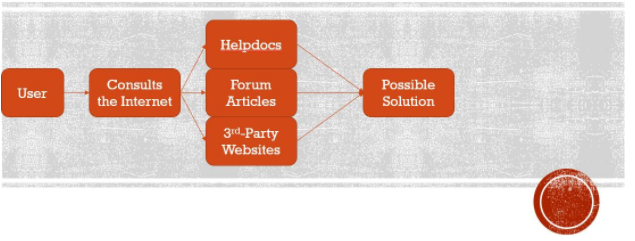
\includegraphics[scale=.75]{option1.png}
		\item Option 2:
		\\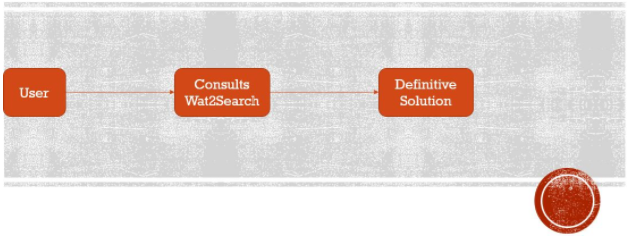
\includegraphics[scale=.75]{option2.png}
	\end{itemize}

	\textbf{Use Cases:}
	
\begin{enumerate}
	\item \textbf{Use Case Name:} Setup Wifi
	\\\textbf{Goal:} Allows a non-technical user to set up or reconnect to their wifi through network preferences
	\\\textbf{Actor:} Non-technical user
	\\\textbf{Preconditions:}
	\begin{itemize}
		\item User owns a device that is able to connect to wifi (example: Macintosh or Windows XP laptop)
		\item Application is designed to assist with the specific device they are using to connect to wifi
		\item A working wifi (private/public) is currently available for use 
		\item User knows their wifi password and wifi name
	\end{itemize}
	\textbf{Postconditions:}
	\begin{itemize}
		\item The wifi is successfully connected, therefore providing internet access to the non-technical user
		\item User verifies with application that they no longer need assistance with this specific problem 
	\end{itemize}
	\textbf{Flow of Events:}
	\begin{itemize}
		\item User is provided instructions/visuals to locate network preferences 
		Example(Windows XP): “Open the Start menu in the bottom left-hand corner of your screen, and then select the Connect To option from the right-hand column.”
		\item User is prompted to select/connect to desired wireless network connection 
		\item Application aids user in navigating network preferences menu by providing visuals highlight specific elements (example: the drop-down menu containing wifi names to select from)
		they might be aided with identifying a wifi available for public use if this is requested by the user
		\item User is guided through process of providing wifi password 
		\item Application validates with the user that they have successfully connected to wifi and will no longer need assistance
	\end{itemize}
	\textbf{Quality Requirements:}
	\begin{itemize}
		\item visuals are high-quality and are efficient in aiding users ability to navigate their computer’s user interface (Example: picture of network preferences menu)
		\item User is able to go back to previous steps when issues arise such as the user chose the wrong wifi network
		\item Instruction wording/diction is simplified in a concise and clear way to ensure the user’s comprehension 
	\end{itemize}

	\item \textbf{Use Case Name:} Reset Password
\\\textbf{Goal:} Allow for an OSU student or staff to reset their ONID password
\\\textbf{Actor:} Non-technical user who is in need of resetting their password
\\\textbf{Preconditions:}
\begin{itemize}
	\item User is an OSU student or staff with a valid ONID username and account
	\item Application is designed to walk them through the resetting process
	\item A working wifi (private/public) is currently available for use 
	\item User knows their ONID username as well as how to use a basic web browser
\end{itemize}
\textbf{Postconditions:}
\begin{itemize}
	\item The specific user is able to print from their personal printer or on-campus OSU printer
	\item User verifies with application that they no longer need assistance with this specific printer problem
\end{itemize}
\textbf{Flow of Events:}
\begin{itemize}
	\item User is provided a link that takes them to the reset password page on OSU’s website
	Example: http://onid.oregonstate.edu/chpw.shtml
	\item User is prompted to select “Login to ONID” if they know their current password 
	\item If the user does not know their password, they are prompted to select the “click here” option below:
	\\Two links may also be provided such as:
	\begin{itemize}
	\item Current password is known:
	\url{https://secure.onid.oregonstate.edu/cgi-bin/my?type=want_auth}
	\item Forgot password:
	\url{https://secure.onid.oregonstate.edu/cgi-bin/chpw?type=want_auth}
	\end{itemize}
	\item The user will be aided with links and screenshots accordingly
	\item User is guided through the reset process and given specific detail on what to enter at every step
	\item Examples are given as well
	\item Application checks with the user if they were successful. If not, a number for tech support and tech support hours will be provided.
\end{itemize}
\textbf{Quality Requirements:}
\begin{itemize}
	\item Visuals are high-resolution and are labeled clearly with important information
	\item User is able to go back to previous steps if an error occurs with resetting their password
	\item Links are kept up to date in order to not provide incorrect or confusing information
	\item Screenshots reflect the most current method to resetting one’s password
\end{itemize}

	\item \textbf{Use Case Name:} Printing Issues
\\\textbf{Goal:} Solve the printing issue for the user and allowing them to print successfully
\\\textbf{Actor:} Non-technical user who is struggling to print either on campus or off
\\\textbf{Preconditions:}
\begin{itemize}
	\item User is non-technical and are unable to print
	\item User is either trying to print on campus or on a personal printer
	\item A working wifi (private/public) is currently available for use 
	\item User knows the basics of operating a web browser
\end{itemize}
\textbf{Postconditions:}
\begin{itemize}
	\item The user was successfully able to print their document
	\item User verifies with application that they no longer need assistance with this specific problem 
\end{itemize}
\textbf{Flow of Events:}
\begin{itemize}
	\item User is prompted to select whether they are trying to print on their own printer or on an OSU printer
	\item If the user selects their own printer, the flowchart will diverge into a separate path
	\item Questions will prompt the user to check if their printer is on, plugged in to power, or plugged in to the computer
	\item Links will be provided to find the appropriate driver for the printer if the user is unsure if the driver has been installed or not
	\\Example:
	Select brand of printer
	\\Link: 
	\url{http://support.brother.com/g/b/productsearch.aspx?c=us&lang=en&content=dl}
	\item The user will be aided with links and screenshots accordingly
	\item User is guided through the install process of the drivers
	\item If that all fails, the user will be prompted to use Windows troubleshooter
	\item Application checks with the user if they were successful. If not, a number for tech support and tech support hours will be provided.
\end{itemize}
\textbf{Quality Requirements:}
\begin{itemize}
	\item Visuals are high-resolution and are labeled clearly with important information
	\item User is able to go back to previous steps if an error occurs with fixing their printer or installing drivers
	\item Links are kept up to date in order to not provide incorrect or confusing information 
\end{itemize}
\end{enumerate}	
The three use cases above cover the most important scenarios for our app Wat2Search. While there are a countless number of scenarios possible, the three we selected are likely the most common to occur. Three of the main issues people have that requires the IT helpdesk is internet connection issues, resetting their ONID password, and issues with printing. The solutions for other problems will be based on these same flow of events. The user will continue to be prompted for questions until a solution is found. In the case of an error, such as the user is unable to understand or follow the directions, we will provide the Helpdesk phone number and hours of operation. This will always be an error case as the Helpdesk is capable of handling more complicated issues that the app may not be able to solve.
\\	
\\\textbf{Planning}
	\\Milestones
	\begin{enumerate}
		\item Documentation 
		\begin{itemize}
			\item Goal: Cover all the potential support info our users may need and work out basic navigation concept.
			\item Timeline: Week 3 - Week 4.
			\item Reasoning: Having all of our goals and use cases set first will allow us to have clear goals when we get to implementation. This will allow us to concentrate on how to incorporate the info we will present to the client during implementation without worrying about what it is. We’ll figure that out in this part of the timeline. 
			\item Reasoning: Having all of our goals and use cases set first will allow us to have clear goals when we get to implementation. This will allow us to concentrate on how to incorporate the info we will present to the client during implementation without worrying about what it is. We’ll figure that out in this part of the timeline. 
		\end{itemize}
		\item Paper Prototype
		\begin{itemize}
			\item Goal: Craft a paper prototype for testers to run through with hypothetical situations clients run into.
			\item Timeline: Week 4 - Week 5.
			\item Testing with the paper prototype: Week 6 - Week 7
			\item Reasoning: Before actually plugging away at the program itself, we want to make that our systems actually make sense to users on a conceptual level. We’ll throw in multiple hypothetical problems to ensure our “dialogue tree” has proper categorization of problems. This is being made or Client Services so we can use staff and student workers for troubleshooting, the extra week for this step allows us to get maximum feedback from our user base. 
			\item Tracking: We can track this by listing the positives and negatives that users have. We’ll know we’re done when we have enough consistent data. We should aim to test at least a handful of participants each. 
		\end{itemize}
	\item Program Prototype
	\begin{itemize}
		\item Goal: Have a functional prototype with the support information integrated for at least basic test cases. 
		\item Timeline: Week 5 - Week 6
		\item Reasoning: With the paper prototype hopefully completed, we can move on to actually seeing how users interact with the widget on their computers. Coding the tree should be easier. We program the most important as well as common problems, determined by the paper prototype, to make sure that the experience of using our app to troubleshoot is solid before implementing the rest. On functionality, we’ll at least add the ability to go between different troubleshooting subjects.
		\item Tracking: We’ll know we’re done with this when we have taken added the most relevant of the data compiled in our documentation. We also  solidified what we need to change from the paper prototype for our user data in the development of the program.
	\end{itemize}
	\item Programming Features
	\begin{itemize}
		\item Goal: Add the rest fo the support doc data into the program. Also add refined navigation through the app
		\item Timeline: Week 7 - Week 8
		\item With the bones of the program in place we can build off of the prototype. We’ll add the entirety of the documented test cases that we deem fit then move on to more advanced functionality like actual integration in multiple browsers as well as different actions for navigation within the network of troubleshooting issues we create for the widget.
		\item Tracking: We can make sure we’re on track for this part by referring to our description of the project in this assignment and making sure our requirements are met. We should also look back on the goals we initially set and look at the program as it is throughout this part of the project.
	\end{itemize}
	\item UI+Graphics
	\begin{itemize}
		\item Goal: Make the program look user friendly and aesthetically pleasing. Finalize the UI with simplicity in mind. 
		\item Timeline: Week 9 - End of term. 
		\item Reasoning: After the program has all of the data needed and is completely functional, we can add visuals to make the program pleasing to the eye. We’re saving this step for last so that we ensure every technical aspect is solid before polishing it to look nice. We’re going with the philosophy that a functional product is more important than one that’s nice to look at. Graphic design and a nice ui will make the client feel more comfortable using it and draw them in, but the actual program will make it reliably used.
		\item Tracking: We need to put this program in front of people and see what they do first to make sure our UI is understandable. For visuals we can debate amongst ourselves and make mini prototypes with powerpoint to test how people respond to different looks. We’ll consider it done once we settle and implement a visual style. 
	\end{itemize}
	\end{enumerate}
	Main Risks:	
	\begin{enumerate}
		\item Lack of Communication: If we aren’t getting input from every member on when and what we’re doing for the development to come we can’t plan ahead. We’re using Discord as our primary means of discussion, an email chain for important matters and we’re going to try to meet up either in person or online for status updates. 
		\item Laziness: In a group project with multiple parts that requires effort from every member this could be one of the deadliest risks. We have to make sure our own initiatives are personally in check so that we can maintain a healthy working relationship with each other. This is just on all of us to make sure we’re sharing work as get this project done at every step of the way.
		\item Losing Scope: This project is meant to be simple in nature. If we give into the “feature creep” discussed in class we’d run the risk of making our troubleshooting app so complex that it needs troubleshooting itself. The best thing we can do is focus and worry about adding anything extra later in the term when we have already met the goals we initially made. 
	\end{enumerate}
\textbf{Meeting Report:}
\\Our progress this week involved setting up our desired communication method and distributing tasks needed to complete this assignment. Initially, we used email to decide our method of communication because we were unable to meet in person from conflicting schedules. We decided to communicate with each other using the mobile application, Discord.  Furthermore, we finished this Software Requirement and Plan(SRP) which includes project information such as our target users and system requirements. This assignment allowed us to test the use of Discord along with Google Doc. 
Next week, we are going to follow our plan and work on it, and we need to have more communication with each other so we can exchange minds more quickly and improve efficiency. 
Through discord and emails we were able to distribute specific tasks to individual members. However, we were unfortunately unable to communicate with our customers to meet with them in person. Though, we were able to make good use of their vision statement and presentation. For example, the vision statement helped in determining use cases that are relevant and should be considered and evaluated for the project.
\\
\bibliography{myref}
\bibliographystyle{plain}

\end{document}
